% ============================================================================
% BLOCK-003 Derivation v5: Normalization Principle Choices to Fix C
% ============================================================================
\documentclass[11pt,a4paper]{article}

\usepackage{fontspec}
\usepackage{amsmath,amssymb,amsthm}
\usepackage{physics}
\usepackage{graphicx}
\usepackage{booktabs}
\usepackage{array}
\usepackage{xcolor}
\usepackage[hidelinks]{hyperref}
\usepackage[margin=2.5cm]{geometry}
\usepackage{fancyhdr}
\usepackage{tikz}
\usetikzlibrary{shapes,arrows,positioning}

% Theorem environments
\newtheorem{lemma}{Lemma}
\newtheorem{proposition}{Proposition}
\theoremstyle{definition}
\newtheorem{definition}{Definition}
\newtheorem{principle}{Normalization Principle}

% Epistemic tags
\newcommand{\BL}{\textsc{[BL]}}
\newcommand{\Ident}{\textsc{[I]}}
\newcommand{\Post}{\textsc{[P]}}
\newcommand{\Deriv}{\textsc{[Dc]}}
\newcommand{\Open}{\textsc{[Open]}}
\newcommand{\Cal}{\textsc{[Cal]}}

% Header/footer
\pagestyle{fancy}
\fancyhf{}
\fancyhead[L]{\small BLOCK-003 / Derivation v5}
\fancyhead[R]{\small EDC Gravity Program}
\fancyfoot[C]{\thepage}

\title{\textbf{BLOCK-003 Derivation v5:}\\[0.3em]
Normalization Principle Choices\\
to Fix $C$ in $\kappa_5^2 = C \cdot \sigma^{-3/4}$}
\author{EDC Working Document}
\date{2026-02-02}

\begin{document}
\maketitle

\begin{abstract}
Derivation v4 proved a No-Go Lemma: the EDC parameters $\{\sigma, \rho_P, R_\xi\}$
provide only two independent scales, insufficient to fix the dimensionless
constant $C$ in $\kappa_5^2 = C \sigma^{-3/4}$.
This note does not close BLOCK-003; instead, it isolates the missing
normalization choice by documenting exactly two candidate principles:
\textbf{NP1} (EDC-internal postulate \Post) fixes $C$ by identifying
$\ell_\sigma = \sigma^{-1/4}$ as the fundamental 5D gravitational length;
\textbf{NP2} (calibrated closure \Cal) fixes $C$ by a single calibration
to the observed Newton constant $G_N^{\rm obs}$.
Both options are presented with their consequences for $G_N$ in the
compact extra dimension scenario.
\end{abstract}

\tableofcontents
\newpage

% ============================================================================
\section{Restatement of the P15 No-Go Result}
% ============================================================================

\begin{lemma}[Dimensional Counting No-Go, from v4]
\label{lem:nogo}
Let the available EDC inputs be $\{\sigma, \rho_P, R_\xi\}$ with the
pressure-balance constraint $\sigma \sim \rho_P \cdot R_\xi^n$.
Then:
\begin{enumerate}
\item The constraint reduces three parameters to two independent scales.
\item The dimensionless $C = \kappa_5^2 \sigma^{3/4}$ requires three
independent scales to be uniquely determined.
\item Therefore, $C$ cannot be fixed from $\{\sigma, \rho_P, R_\xi\}$
alone without an additional normalization principle.
\end{enumerate}
\end{lemma}

\noindent
\textbf{Status:} Proven in derivation v4. This note assumes the No-Go
and explores resolution paths.

% ============================================================================
\section{The Normalization Fork}
% ============================================================================

The No-Go lemma implies that closing $\kappa_5^2$ requires exactly one
additional input. We identify two clean options:

\begin{figure}[h]
\centering
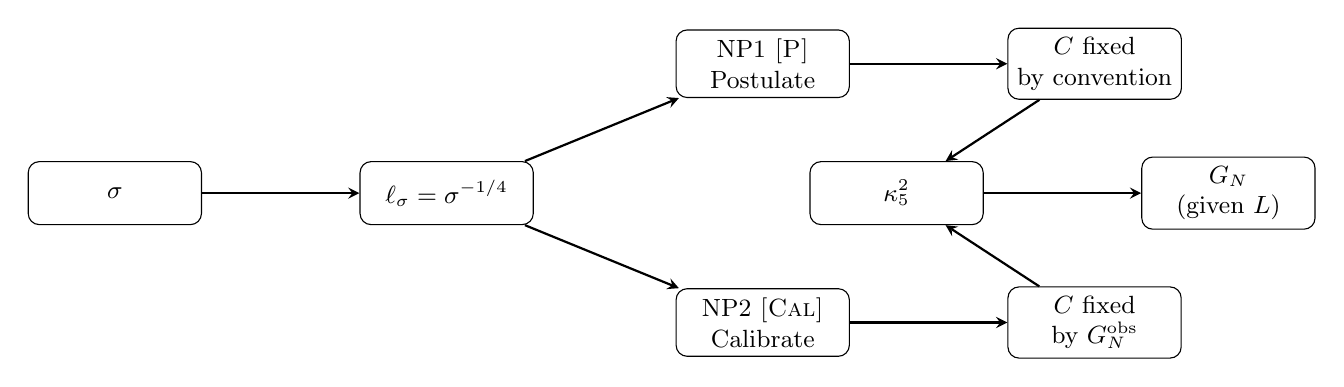
\begin{tikzpicture}[
    node distance=1.2cm and 2.0cm,
    box/.style={rectangle, draw, rounded corners, minimum width=2.2cm,
                minimum height=0.8cm, align=center, font=\small},
    arrow/.style={->, >=stealth, thick}
]
% Nodes
\node[box] (sigma) {$\sigma$};
\node[box, right=of sigma] (ell) {$\ell_\sigma = \sigma^{-1/4}$};
\node[box, above right=0.8cm and 1.8cm of ell] (np1) {NP1 \Post\\Postulate};
\node[box, below right=0.8cm and 1.8cm of ell] (np2) {NP2 \Cal\\Calibrate};
\node[box, right=of np1] (c1) {$C$ fixed\\by convention};
\node[box, right=of np2] (c2) {$C$ fixed\\by $G_N^{\rm obs}$};
\node[box, right=3.5cm of ell] (kappa) {$\kappa_5^2$};
\node[box, right=of kappa] (gn) {$G_N$\\(given $L$)};

% Arrows
\draw[arrow] (sigma) -- (ell);
\draw[arrow] (ell) -- (np1);
\draw[arrow] (ell) -- (np2);
\draw[arrow] (np1) -- (c1);
\draw[arrow] (np2) -- (c2);
\draw[arrow] (c1) -- (kappa);
\draw[arrow] (c2) -- (kappa);
\draw[arrow] (kappa) -- (gn);
\end{tikzpicture}
\caption{Schematic of the normalization fork. From brane tension $\sigma$,
the length scale $\ell_\sigma$ emerges. Two principles can fix the
dimensionless $C$: NP1 by postulate, NP2 by calibration. Either path
yields $\kappa_5^2$, which combined with compactification length $L$
gives $G_N$. \textit{Schematic; not a result.}}
\label{fig:fork}
\end{figure}

% ============================================================================
\section{NP1: EDC-Internal Postulate}
\label{sec:np1}
% ============================================================================

\begin{principle}[NP1: Identification Postulate \Post]
\label{np1}
The tension-derived length scale $\ell_\sigma = \sigma^{-1/4}$ is identified
as the fundamental 5D gravitational length $\ell_5$, with the standard
gravitational normalization:
\begin{equation}
\kappa_5^2 = 8\pi \ell_5^3 = 8\pi \ell_\sigma^3 = 8\pi \sigma^{-3/4}
\label{eq:np1}
\end{equation}
\end{principle}

\subsection{Consequences of NP1}

Under NP1, the constant $C$ is fixed by convention:
\begin{equation}
\boxed{C = 8\pi}
\end{equation}

The 4D Newton constant (for compact extra dimension of size $L$) becomes:
\begin{equation}
G_N = \frac{\kappa_5^2}{6\pi L} = \frac{8\pi \sigma^{-3/4}}{6\pi L}
= \frac{4}{3} \cdot \frac{\sigma^{-3/4}}{L}
\label{eq:gn_np1}
\end{equation}

\subsection{Epistemic Status}

\begin{itemize}
\item \textbf{Tag:} \Post\ (postulate, not derived)
\item \textbf{What it assumes:} $\ell_\sigma$ is the natural 5D Planck length
in EDC; the factor $8\pi$ follows standard GR normalization convention.
\item \textbf{What remains open:} The compactification length $L$ must still
be specified. If $L = R_\xi$ \Post, then:
\begin{equation}
G_N^{\rm NP1} = \frac{4}{3} \cdot \frac{\sigma^{-3/4}}{R_\xi}
\quad \text{\Post}
\label{eq:gn_np1_rxi}
\end{equation}
\end{itemize}

\subsection{Predictivity}

Under NP1 + $L = R_\xi$, $G_N$ is determined by $\sigma$ and $R_\xi$ alone.
The model becomes predictive \textit{if} $\sigma$ can be computed from
EDC field equations (currently \Open).

% ============================================================================
\section{NP2: Calibrated Closure}
\label{sec:np2}
% ============================================================================

\begin{principle}[NP2: Single Calibration \Cal]
\label{np2}
The constant $C$ is fixed by requiring that the resulting $G_N$ matches
the observed value $G_N^{\rm obs} = 6.674 \times 10^{-11}\,\text{m}^3
\text{kg}^{-1}\text{s}^{-2}$ for a specified $L$.
\end{principle}

\subsection{Consequences of NP2}

From $G_N = \kappa_5^2 / (6\pi L)$ and $\kappa_5^2 = C \sigma^{-3/4}$:
\begin{equation}
G_N^{\rm obs} = \frac{C \sigma^{-3/4}}{6\pi L}
\end{equation}

Solving for $C$:
\begin{equation}
\boxed{C = 6\pi L \cdot G_N^{\rm obs} \cdot \sigma^{3/4}}
\label{eq:c_np2}
\end{equation}

\subsection{Epistemic Status}

\begin{itemize}
\item \textbf{Tag:} \Cal\ (calibrated, not first-principles)
\item \textbf{What it assumes:} One empirical input ($G_N^{\rm obs}$) is
used to fix the normalization. This is operationally legitimate but not
a derivation.
\item \textbf{What remains open:} The compactification length $L$ appears
in the calibration. If $L = R_\xi$ \Post, then:
\begin{equation}
C = 6\pi R_\xi \cdot G_N^{\rm obs} \cdot \sigma^{3/4}
\quad \text{\Cal}
\label{eq:c_np2_rxi}
\end{equation}
\end{itemize}

\subsection{Predictivity}

Under NP2, $G_N$ is \textit{not} predicted---it is input. However, the
calibration makes other gravitational observables (e.g., corrections to
Newtonian potential, brane-world signatures) predictive, conditional on
the model structure.

\textbf{Key distinction:} NP2 does not claim to derive $G_N$; it uses
$G_N^{\rm obs}$ once to close the system, then explores consequences.

% ============================================================================
\section{Comparison Table}
% ============================================================================

\begin{table}[h]
\centering
\begin{tabular}{lll}
\toprule
\textbf{Aspect} & \textbf{NP1 (Postulate)} & \textbf{NP2 (Calibration)} \\
\midrule
Tag & \Post & \Cal \\
Fixes $C$ by & Convention ($8\pi$) & Empirical input ($G_N^{\rm obs}$) \\
$G_N$ status & Predicted (if $\sigma$ known) & Input \\
Falsifiable? & Yes (if $\sigma$ computed) & No (by construction) \\
EDC-internal? & Yes & Partially (uses external data) \\
Requires $L$? & Yes (e.g., $L = R_\xi$ \Post) & Yes (enters calibration) \\
\bottomrule
\end{tabular}
\caption{Comparison of normalization principle options.}
\label{tab:compare}
\end{table}

% ============================================================================
\section{What This Note Does Not Do}
% ============================================================================

This note explicitly does \textbf{not}:

\begin{enumerate}
\item \textbf{Close BLOCK-003.} The gravity sector remains open because
neither NP1 nor NP2 is derived from EDC field equations.

\item \textbf{Derive $C$ from first principles.} Both options involve
either postulating a convention (NP1) or using empirical input (NP2).

\item \textbf{Specify $L$.} The compactification length remains symbolic
unless separately postulated as $L = R_\xi$ or derived from EDC geometry.

\item \textbf{Prefer one option over the other.} The choice between NP1
and NP2 is a modeling decision, not a mathematical necessity.
\end{enumerate}

\textbf{What this note does:} It isolates the exact missing element
(one normalization principle) and presents the two cleanest options
available within the current EDC framework.

% ============================================================================
\section{Path Forward}
% ============================================================================

To truly close BLOCK-003 without postulate or calibration, one would need:

\begin{enumerate}
\item \textbf{A derived normalization} \Deriv: An EDC mechanism that
produces a specific numerical prefactor (e.g., topological quantization,
$\mathbb{Z}_6$ symmetry constraint, or holographic bound).

\item \textbf{A derived $L$} \Deriv: An EDC equation that determines the
compactification scale from internal geometry (e.g., $L$ from membrane
thickness $\delta$ or bulk curvature).
\end{enumerate}

Until such derivations exist, NP1 or NP2 represent the available options
for operational closure.

% ============================================================================
\section{Summary}
% ============================================================================

\begin{center}
\fbox{\parbox{0.9\textwidth}{
\textbf{Outcome:} Two normalization principle options documented.
\begin{itemize}
\item \textbf{NP1} \Post: $\kappa_5^2 = 8\pi \sigma^{-3/4}$ (convention)
$\Rightarrow$ $G_N = \frac{4}{3} \sigma^{-3/4} / L$
\item \textbf{NP2} \Cal: $C = 6\pi L \cdot G_N^{\rm obs} \cdot \sigma^{3/4}$
(calibration) $\Rightarrow$ $G_N = G_N^{\rm obs}$ by construction
\end{itemize}
\textbf{BLOCK-003 remains OPEN} pending a derived normalization principle.
}}
\end{center}

\end{document}
